% author: Man Cao, Lilong Jiang
\documentclass{article}
\usepackage[letterpaper]{geometry} \usepackage[utf8]{inputenc}
\usepackage[T1]{fontenc}
\usepackage{amsmath}
\usepackage{hyperref}
\usepackage{relsize}
\usepackage{graphicx}

\newcommand{\code}[1]{\textsf{\smaller\verb~#1~}}

\begin{document}

\title{CSE5243 Assignment 4}
\author{Man Cao(cao.235), Lilong Jiang(jiang.573)}
\maketitle

\section{Work Separation}
Lilong mainly worked on hierarchical clustering. Man mainly worked on
K-means. In fact there were a lot of overlapping during the
work, we exchanged various ideas and wrote the this report together.
\section{Input}
After eliminating documents without topics, 11367 documents are left.\\
The input file has the following format:
\begin{verbatim}
{'NEWID':<value>, 'TOPICS':[value1, value2, ...], 'PLACES':[value1, value2, ...]}
{<term1>:<value1>, <term1>:<value2>, ...}
\end{verbatim}
Note that each document corresponds to two lines: the first line contains the
metadata of the document, the second line is the frequency vector.

\section{Metrics}
Cosine similarity and Jaccard similarity are used in this assignment.

\section{Algorithms}
\subsection{Hierarchical Clustering}
\subsubsection{Single Link}
We use the single-link to define the inter-cluster similarity. In every
iteration, the two clusters with minimum distance will be merged.
\subsubsection{Implemtation Details}
Since the similarity between cluster1 and cluster2 is the same as the similarity
between cluster2 and cluster1, we only need to store the \emph{upper triangle of
the matrix}.

Also considering the expensive time complexity of finding the min distance in
the matrix, we transform the proximity matrix to a proximity list and
\emph{sort} the list before clustering. In this way, we only check the
distance from the last position. For every document, we records which cluster it
belongs to and for every cluster, we record which documents are in it.

The sorting time for the proximity list is $O(N^2logN)$, since there exist
$\frac{N^2}{2}$ elements in the list, where $N$ is the number of documents.
There are N iterations in total and in every iteration, we need to find the next
minimum distance and update the mapping relationship between the documents and
clusters. The time complexity of finding the next minimum distance and updating
the mapping relationship in N iterations is $O(N^2)$, so the total time
complexity is $O(N^2logN)$.
\subsection{K-means Clustering}
We implement the na\"ive K-means algorithm as described in the slides from
class:
\begin{enumerate}
  \item Randomly select K distinct documents as the initial centroids of K
  clusters.
  \item \label{repeat} For each document, compute similarities between the
  document and each of the K centroids; assign the document to the cluster whose
  centroid has largest similarity with the document.
  \item For each cluster, recompute its centroid, which is the mean of all
  documents in the cluster; also compute the distance between the new centroid
  and old centroid.
  \item If, for any cluster, the distance between the new centroid and old
  centroid is greater than thresold value, repeat from step~\ref{repeat}. 
\end{enumerate}

\noindent The distance between two documents d1 and d2 is simply $1.0 -
similarity(d1, d2)$. In our experiment, the threshold value is 0.001. We did not
encounter the empty cluster problem during our experiment.

Interestingly, we observed that it is possible that K-means does not converge.
In one case, we ran K-means for nearly 40 hours with K=16 and cosine similarity,
and it did not give an output. Then we ran it again with the same configuration,
and it just finished in 35 minutes.

We found proof states that for large scale of data, it is quite possible for
K-means to oscillate between two or more partitions and never converge
\footnote{\url{http://www.clustan.com/k-means_critique.html\#FailureToConverge}}
\footnote{``Some methods for classification and analysis of multivariate
observations'', MacQueen, Berkeley Symposium, 1967, p. 288}. One solution is to
compute the variance of Sum of Squared Error (SSE) every time the algorithm
tries to move an element to a different cluster, considering the slight change
of the centroids of the two involved clusters. If such movement can reduce the
SSE, then move it; otherwise do not move the element. We did not implement this
approach, because it should be much slower, and we do not see the oscillation
case very often.
%This approach is to directly minimize the SSE for every step, thus can avoid
% the oscillation. However, it is definitely more expensive than the na\"ive K-means,
% and shares some similarity to the incremental updating centroids approach.

\section{Evaluation}

The evaluation is performed on a Linux instance purchased on Amazon Elastic
Compute Cloud (Amazon EC2). It is a node of the type ``large" with 2.4GHz
CPU and 17.1GB main memory. We chose to run on EC2 mainly because hierarchical
clustering has a rather large memory footprint that stdlinux is no longer
suitable.

Our evaluation is only based on the first 2500 documents, because Hierarchical
Clustering is so slow that it cannot finish for 11367 documents within a
reasonable amount of time (the estimated time is around 48 hours). Although
K-means can finish for the 11367 documents within 10 hours (we have the result),
we show the result of K-means for 2500 documents, in order to properly compare
the two algorithms.

\subsection{Scalability}
The time for clustering 2, 4, 8, 16 and 32 clusters with Hierarchical Clustering
and K-means is show in Fig~\ref{Fig:scalability}. Actually it does not make good
sense to compare the execution time in this way. Hierarchical Clustering only
needs to compute the dendrogram once, and use the same dendrogram for any number
of clusters. K-means needs to recompute from scratch, if the number
of clusters changes. The result in the figure for Hierarchical actually
includes the time to build the dendrogram, for each number of clusters.

\begin{figure}
\centering
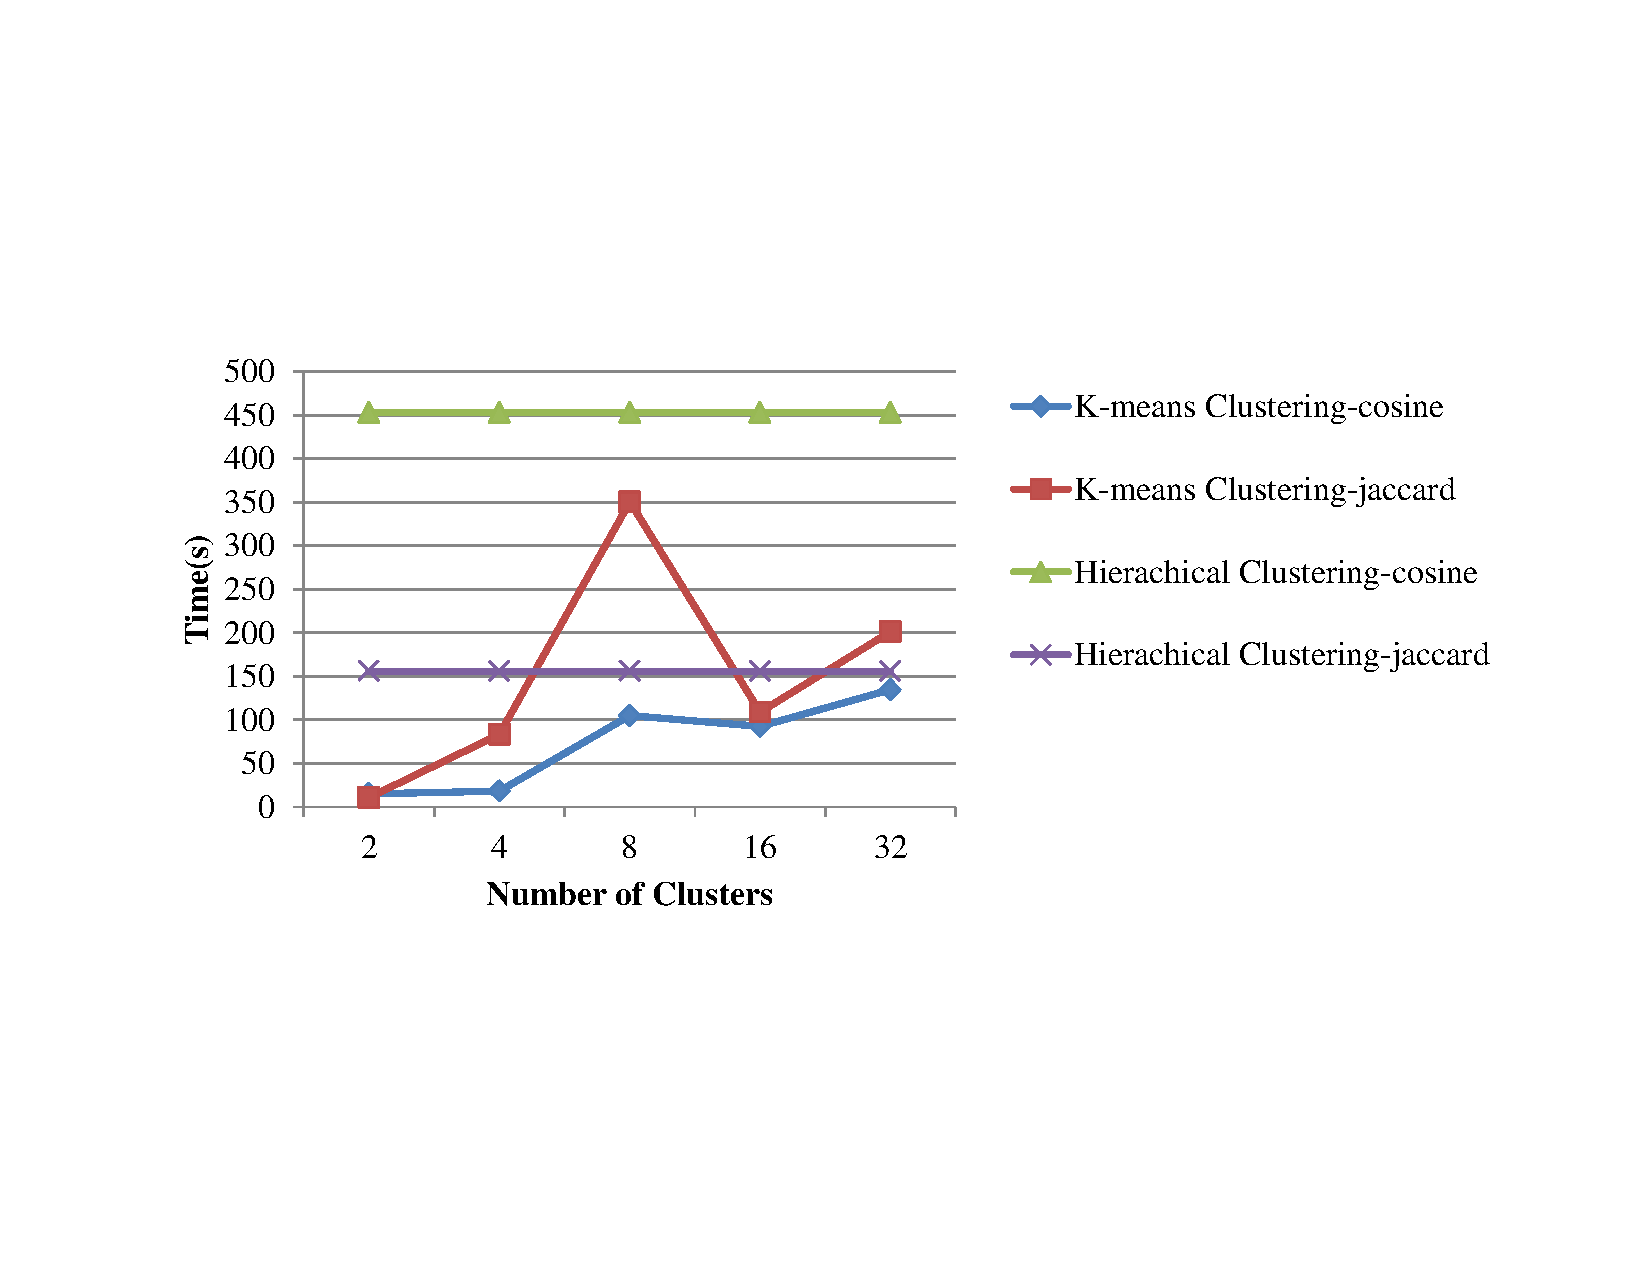
\includegraphics[width=0.8\textwidth]{Scalability}
\caption{\footnotesize Execution time of Hierarchical and K-means clustering
with Cosine and Jaccard similarities.}
\label{Fig:scalability}
\end{figure}
\subsection{Quality}
\subsubsection{Entropy}
For a document with multiple topics, each topic receives a \emph{vote} of
$1/n$, where $n$ is the number of topics in the document. The probability of a
topic $t$ within a cluster $C_x$ is then:
\begin{equation}
P(t|C_x)=\frac{\sum_{docs}v_{it}}{\sum_{docs}\sum_{topics}v_{ij}}
\end{equation}
where $v_{ij}$ is the vote of topic $j$ from document $i$.

In order to make sure the entropy falls within the range of $[0, 1.0]$, we use
$m$ as the base of the logarithm, where $m$ is the number of distinct topics in
the cluster. That is:
\begin{equation}
m = |C_x.topics|
\end{equation}

The entropy of the clustering is the sum of weighted entropy of each cluster. 

Figure~\ref{Fig:entropy} shows the entropy of the clustering. For
K-means, we can clearly see the decrease in entropy, as the number of clusters
increases. However, for Hierarchical, such effect is not so obvious. We presume
the reason is that there are outliers in the input, and we did not
explicitly handle them; meanwhile, single-link hierarchical clustering is more
susceptible to outliers than K-means.

\begin{figure}
\centering
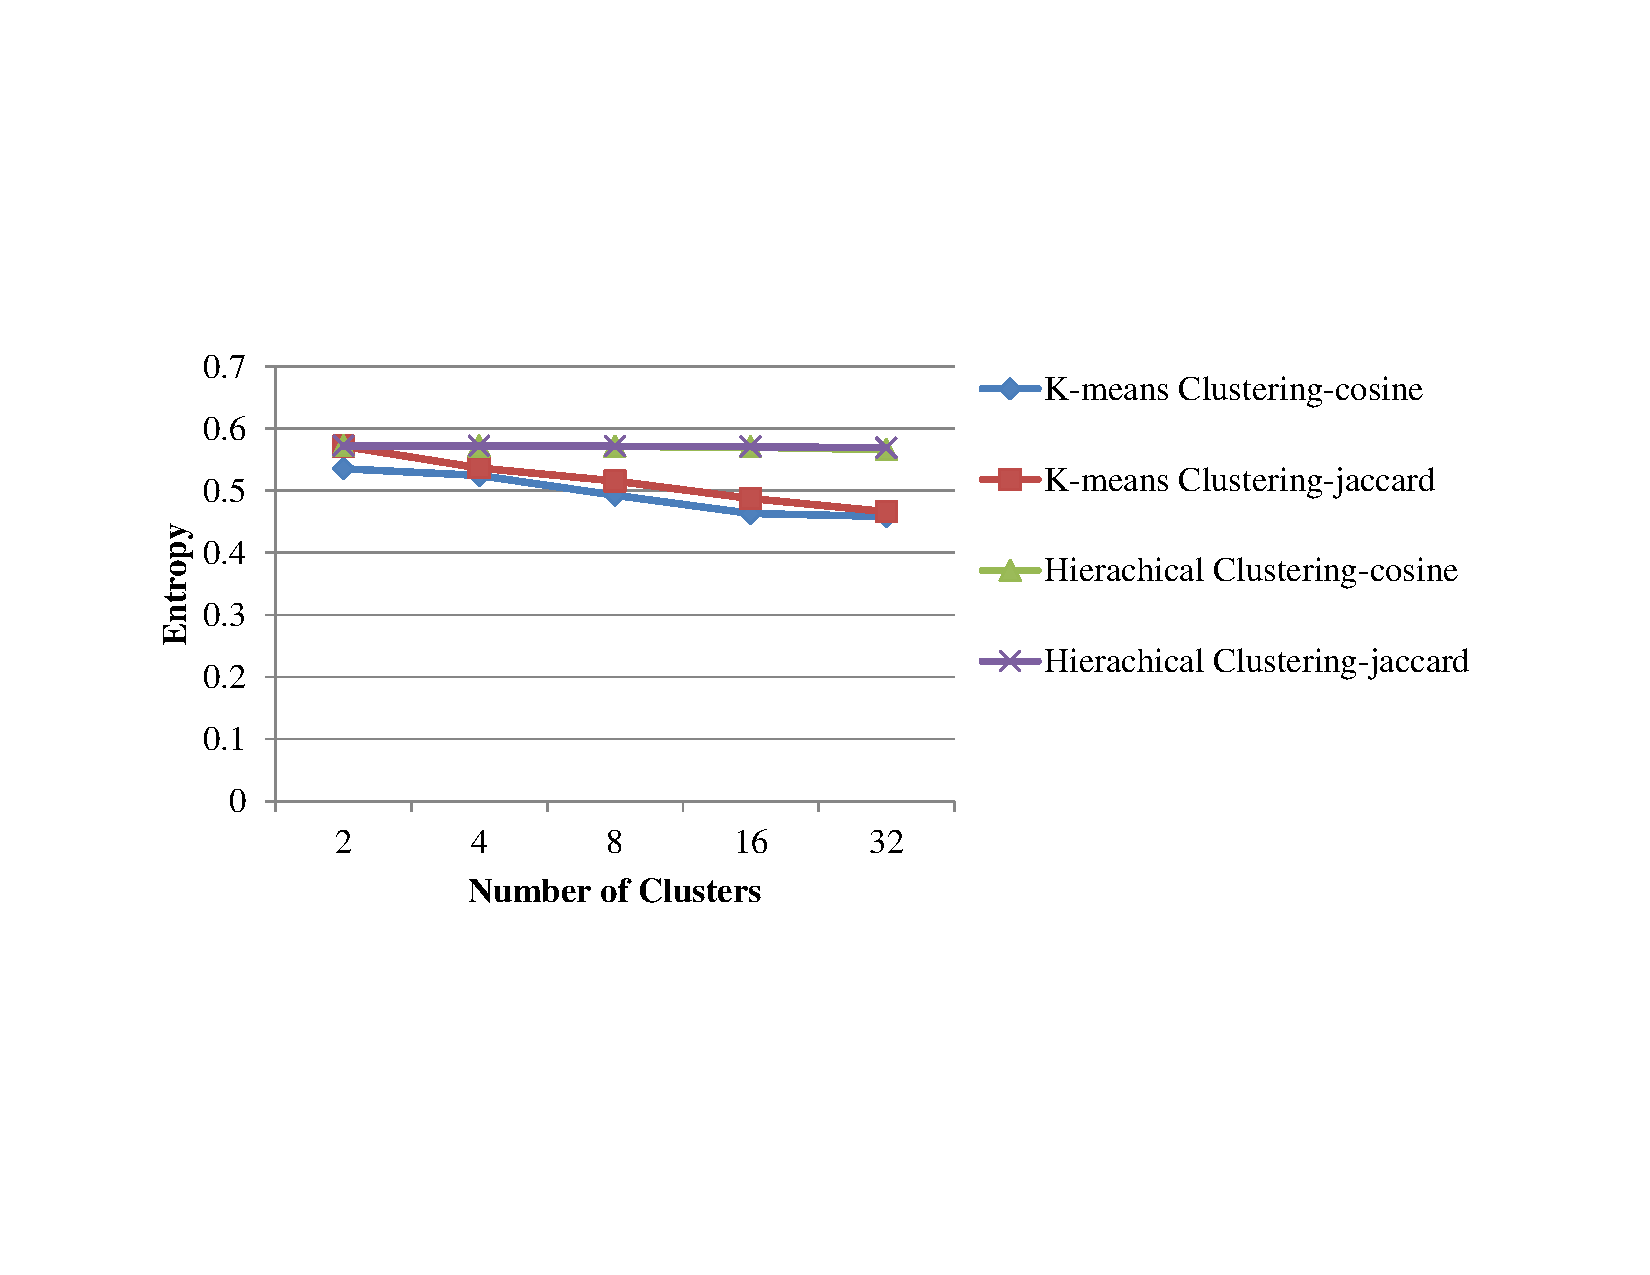
\includegraphics[width=0.8\textwidth]{Entropy}
\caption{\footnotesize The entropy of the clustering for Hierarchical and K-means
with Cosine and Jaccard similarities.}
\label{Fig:entropy}
\end{figure}

\subsubsection{Skew}
The skew is measured as variance of the cardinalities of different clusters.
In Figure~\ref{Fig:skew}, we can clearly see the skew decreases as the number of
clusters increases, for both clustering algorithms.

We can argue that Cosine similarity is better that Jaccard for text data, since
both entropy and skew are lower with Cosine similarity.
\begin{figure}[b!]
\centering
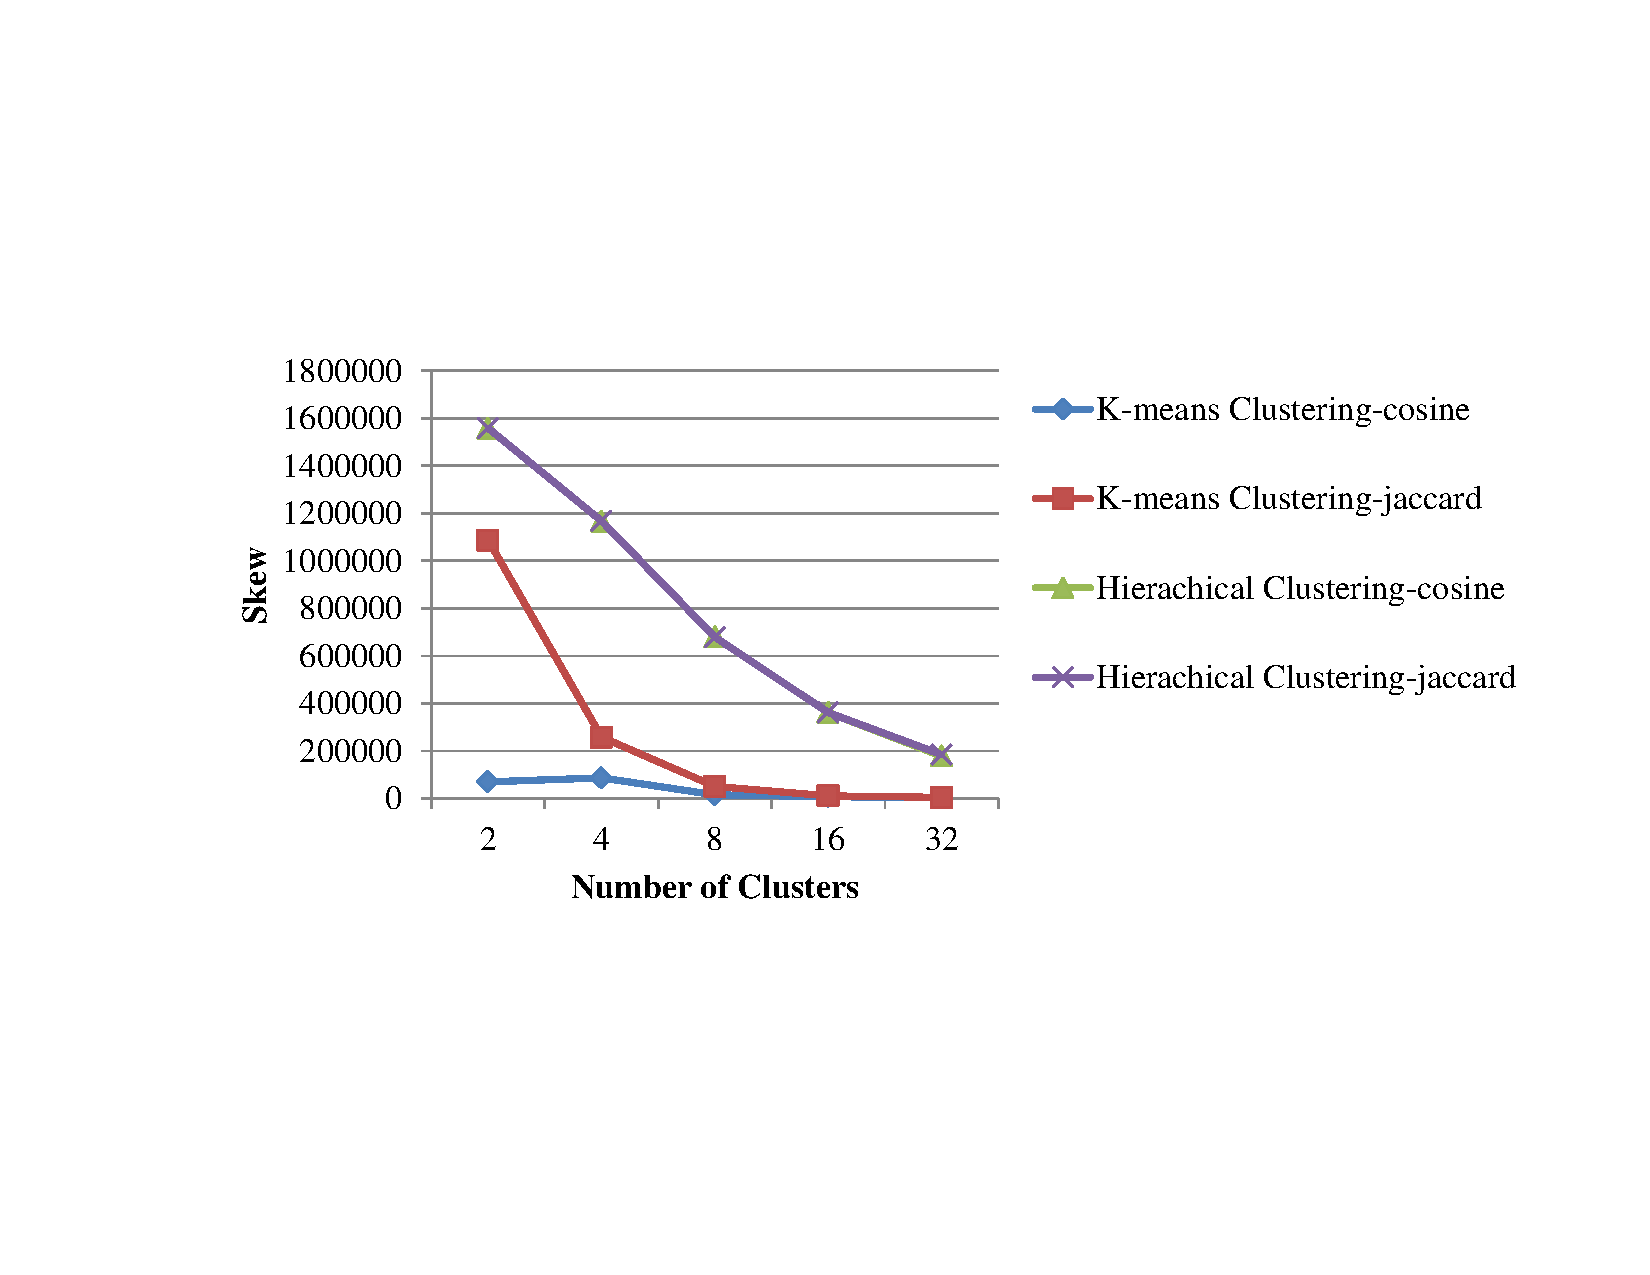
\includegraphics[width=0.8\textwidth]{Skew}
\caption{\footnotesize The skew of the clustering for Hierarchical and K-means
with Cosine and Jaccard similarities.}
\label{Fig:skew}
\end{figure}
\end{document}
